\documentclass{memoir}
\usepackage{amssymb,amsmath,mathtools}


\usepackage{algorithm2e,algorithmic}

\usepackage{mathrsfs}
\usepackage{paralist}

\usepackage{esint} % for \fint

\allowdisplaybreaks

\usepackage{color}		% enable color characters
\usepackage{graphicx} 	% insert image files
\usepackage{enumerate} 	% enumerate items
\usepackage{caption}
\usepackage{subcaption}
\usepackage{multirow,multicol}
\usepackage[makeroom]{cancel}

\usepackage[colorlinks=true,linkcolor=blue,citecolor=blue]{hyperref}

\usepackage{makeidx}

\newcommand{\cem}[1]{\color{magenta}{\em{#1}}} % color emphasize
\newcommand{\dual}[2]{{#1}^{(#2)}} % color emphasize

\newcommand{\tr}{{\mathrm{tr}}}
\renewcommand{\vec}{{\mathrm{vec}}}

\newcommand{\dd}{{\,\mathrm{d}\,}}
%%
%% horizontal and vertical centering in table p mode
%%
\usepackage{array}
\newcolumntype{P}[1]{>{\centering\arraybackslash}p{#1}} % horizontal centering
\newcolumntype{M}[1]{>{\centering\arraybackslash}m{#1}} % vertical centering

%%
%% define bold font for the alphabet
%%
\usepackage{pgffor}
\foreach \letter in {a,...,z}{ % bold font for a..z
\expandafter\xdef\csname \letter \endcsname{\noexpand\ensuremath{\noexpand\mathbf{\letter}}}
}
\foreach \letter in {A,...,Z}{ % bold font for A..Z
\expandafter\xdef\csname \letter \endcsname{\noexpand\ensuremath{\noexpand\mathbf{\letter}}}
}
\foreach \letter in {A,...,Z}{ % `field' font for AA..ZZ
\expandafter\xdef\csname \letter\letter \endcsname{\noexpand\ensuremath{\noexpand\mathcal{\letter}}}
}
\foreach \letter in {A,...,Z}{ % `field' font for AAA..ZZZ
\expandafter\xdef\csname \letter\letter\letter \endcsname{\noexpand\ensuremath{\noexpand\mathbb{\letter}}}
}
\newcommand{\balpha}{{\boldsymbol{\alpha}}}
\newcommand{\bbeta}{{\boldsymbol{\beta}}}
\newcommand{\bgamma}{{\boldsymbol{\gamma}}}
\newcommand{\bkappa}{{\boldsymbol{\kappa}}}
\newcommand{\bmu}{{\boldsymbol{\mu}}}
\newcommand{\btheta}{{\boldsymbol{\theta}}}
\newcommand{\bTheta}{{\boldsymbol{\Theta}}}
\newcommand{\bPi}{{\boldsymbol{\Pi}}}
\newcommand{\bSigma}{{\boldsymbol{\Sigma}}}
\newcommand{\bPhi}{{\boldsymbol{\Phi}}}
\newcommand{\bLambda}{{\boldsymbol{\Lambda}}}
\newcommand{\bdeta}{{\boldsymbol{\eta}}}
\newcommand{\bphi}{{\boldsymbol{\phi}}}



%%
%% add definitions and theorems
%%
\usepackage[thmmarks,amsmath]{ntheorem}
\theorembodyfont{\normalfont}
\newtheorem{deff}{Definition}[section]
\newtheorem{thm}{Theorem}[section]
\newtheorem{prop}{Proposition}[section]
\newtheorem{lem}{Lemma}[section]
\newtheorem{cor}{Corollary}[section]
\newtheorem{rmk}{Remark}[section]
\newtheorem{alg}{Algorithm}[section]
\newtheorem{ex}{Example}[section]
\newtheorem{ques}{Question}[section]
\newtheorem{ans}{Answer}[section]
\newtheorem{prob}{Problem}[section]
\newtheorem{sol}{Solution}[section]
\newtheorem*{prof}{Proof}[section] 

\title{Probability}
\author{Xi Tan (tan19@purdue.edu)}
\date{\today}

\begin{document}
\maketitle
\tableofcontents

\newpage
\chapter*{Preface}
This booklet is divided into 7 Chapters. The first chapter introduces the definitions of basic concepts, such as event, sample space, and probability space. Followed in the next chapter, we will discuss the relationship between two or more events when they interplay with each other. The third chapter formally brings in random variables and vectors, as a basis to develop their quantitative measure and characteristic functions later in chapter four. Chapter five includes some well-known limit theorems, which is useful for asymptotic analysis. The last two chapters will discuss several selected topics in probability theory, and provide a summary of common distributions.

\newpage
\part{Elementary Theory of Probability}
\section{Combinatorial Analysis}
\section{Axioms}
There are two important rules in combinatorics: the rule of sum, and the rule of product.

The rule of sum says, if we have $a$ ways to finish a task using one method and alternatively, $b$ ways to finish the same task using another method, then there are $ab$ ways of finish this task. More generally,
\begin{equation}
	|S_1 \cup S_2 \cup \ldots \cup S_n| = |S_1| + |S_2| + \ldots + |S_n|
\end{equation}

One extension of the rule of sum is the inclusion-exclusion principle, which does not require sets $A_i$ to be disjoint. This does include the rule of sum, in that if sets $A_i$ are disjoint, the terms from the second to the last are all zero.
\begin{equation}
\begin{split}
|\bigcup_{i=1}^n A_i| = & \sum_{i=1}^n|A_i| - \sum_{1 \le i < j \le n}|A_i\cap A_j| + \sum_{1 \le i < j < k \le n}|A_i\cap A_j\cap A_k|-\ \cdots\ \\
&  +  \left(-1\right)^{n-1} |A_1\cap\cdots\cap A_n|
\end{split}
\end{equation}

The rule of product says, if finishing one task requires two steps, and there are $a$ ways to choose in the first step and $b$ ways to choose in the second step, then there are $ab$ ways to finish this task. More generally,
\begin{equation}
|S_1 \times S_2 \times \cdots \times S_n| = |S_{1}| \cdot |S_{2}| \cdots |S_{n}|
\end{equation}

\section{Binomial Coefficient and Its Applications}
\subsection{Binomial Coefficient}
We list here some of the useful binomial identities, all numbers are nature number (not including 0).

\begin{equation}
	{n \choose k} = {n \choose n-k}
\end{equation}

\begin{equation}\label{eq:subset_count}
	\sum^n_{k=0} {n \choose k} = 2^n
\end{equation}

\begin{equation}
	{n \choose k} = \frac{n}{k}{n-1 \choose k-1}
\end{equation}

\noindent{From the famous Pascal's rule,}
\begin{equation}\label{eq:Pascal's_rule}
	{n \choose k} + {n \choose k+1} = {n+1 \choose k+1}
\end{equation}
There is another form which is equivalent to equation \ref{eq:Pascal's_rule},
\begin{equation}
	{n \choose k} = {n-1 \choose k-1} + {n-1 \choose k}
\end{equation}

\noindent Here is an example that uses the {\em{logarithmic differentiation}}, $f' = f \dot [\ln(f)]'$.
\begin{equation}
	\frac{d}{dt} {t \choose k} = {t \choose k} \sum^{k-1}_{i=0} \frac{1}{t-i}
\end{equation}

\noindent A list of series that involves binomial coefficients,
\begin{eqnarray}
	\sum^n_{k=0} {n \choose k} = 2^n \\
	\sum^n_{k=0} k {n \choose k} = n 2^{n-1} \\
	\sum^n_{k=0} k^2 {n \choose k} = (n+n^2) 2^{n-2}
\end{eqnarray}
These can all be obtained by examining the function value or derivatives of the function $(1+x)^\alpha$, where $\alpha$ could be any real number, and $|x| < 1$.

There are some identities that could be proved using combinatorial analysis, such as {\em{double counting}}. Here is an example,
\begin{equation}\label{eq:double_count}
	\sum^n_{k=1} {n \choose k} {k \choose q} = 2^{n-q} {n \choose q}
\end{equation}
The left side of equation \ref{eq:double_count} counts the number of ways of selecting $k$ elements first, and then choosing $q$ elements from the resulting subset. These $q$ elements could be identical for different $k$. The right hand side of the equation says this is equivalent to first choosing $q$ elements directly from the set, and merging them into one of the $2^{n-q}$ subset of the set containing all but those selected $q$ elements.

Another example is,
\begin{equation}
	\sum^{n_1}_{m_1=0} {n_1 \choose m_1} {n_2 \choose m-m_1} = {n \choose m}
\end{equation}
This simply means choosing $m=m_1+m_2$ objects from a set of $n=n_1+n_2$ objects is equivalent to choosing $m_1$ objects from $n_1$ objects, and $m_2$ objects from $n_2$ objects.

Sometimes, knowing the bounds and asymptotic formulae could be helpful.
\begin{equation}
	\left(\frac{n}{k}\right)^k \le {n \choose k} \le {\frac{n^k}{k!}} \le \left(\frac{n \cdot e}{k}\right)^k
\end{equation}

\begin{equation}
	{2n \choose n} \sim \frac{4^n}{\sqrt{\pi n}}, \mbox{ as } n \rightarrow \infty
\end{equation}

\subsection{Bernoulli Distribution}
\subsection{The i.i.d. Case: Binomial Distribution}
\subsection{The Batch Mode Case: Hypergeometric Distribution}



\section{Multinomial Coefficient and Its Applications}

\subsection{Multinomial Coefficient}
The notion of {\em{multinomial coefficient}} is a generalization of binomial coefficient, which is defined in the multinomial theorem:
\begin{equation*}
	(x_1+x_2+\ldots+x_r)^n = \sum_{(n_1,\ldots,n_r):n_1+\ldots,n_r=n} {n \choose n_1,n_2,\ldots,n_r}x_1^{n_1}x_2^{n_2} \ldots x_r^{n_r}
\end{equation*}
We call $n \choose n_1,n_2,\ldots,n_r$ the multinomial coefficient.

\begin{prob}
	A set of $n$ distinct items is to be divided into $r$ distinct groups of respective sizes $n_1, n_2, \ldots, n_r$, where $\sum^r_{i=1} n_i = n$. How many different divisions are possible?
\end{prob}
Note that there are $n \choose n_1$ possible choices for the first group; for each choice of the first group there are $n \choose n-n_1$ possible choices for the second group; and so on. Hence it follows that there are
\begin{equation*}
\begin{split}
	& {n \choose n_1} {n-n_1 \choose n_2} \ldots {n-n_1-n_2- \ldots -n_{r-1} \choose n_r} \\
	& = \frac{n!}{(n-n_1)!n_1!} \frac{(n-n_1)!}{(n-n_1-n_2)!n_2!} \ldots \frac{(n-n_1-n_2- \ldots -n_{r-1}!}{(0)!n_r!} \\
	& = \frac{n!}{n_1!n_2! \ldots n_r!}
\end{split}
\end{equation*}
possible divisions.

Alternatively, we can first permute these $n$ items, where there are $n!$ such orderings. The first $n_1$ elements are assigned to group $1$, the next $n_2$ elements are assigned to group $2$, and so on. However, for example, keeping all but $n_i$ group fixed, this method would generate $n_i!$ equivalent divisions (note the order within a group does not matter). Therefore, we need to cancel out the equivalent-group effect by dividing $n_1!n_2! \ldots n_r!$. Finally, the multinomial coefficient is,
\begin{equation}
	{n \choose n_1,n_2,\ldots,n_r} = \frac{n!}{n_1!n_2! \ldots n_r!}
\end{equation}

\section{Categorical Distribution}
\section{Multinomial Distribution}


\section{Multiset Coefficient and Its Applications}
\subsection{Multiset Coefficient}
The notion of multiset (or bag) is a generalization of the notion of set in which members are allowed to appear more than once.

The number of times an element belongs to the multiset is the {\em{multiplicity}} of that member. The total number of elements in a multiset, including repeated memberships, is the {\em{cardinality}} of the multiset. For example, in the multiset \{a, a, b, b, b, c\} the multiplicities of the members a, b, and c are respectively 2, 3, and 1, and the cardinality of the multiset is 6.

The number of multisets of cardinality $k$, with elements taken from a finite set of cardinality $n$, is called the {\em{multiset}} coefficient or {\em{multiset number}}, and is denoted as $\left(\!\!{n\choose k}\!\!\right)$. It is equivalent to asking, with replacement, the number of all possible combinations of making $k$ draws from a urn with $n$ distinguishable balls labeled $1 \dots n$.

\begin{prob}\label{prob:multiset}
	With replacement, how many possible combinations to make $k$ draws from a urn with $n$ distinguishable balls labeled $1 \dots n$?
\end{prob}
%If we translate this prob directly to the combinatorial language, \smallmarginpar{It is NOT the sum of all the multinomial coefficients, which can be seen by computing $(1+ \dots +1)^k$, that is, $\sum {k \choose N_1, N_2, \ldots, N_n} = n^k$.} we may end up with counting the total number of the multinomial coefficients (actually, it is also correct). To solve this prob, let's first see a similar example.

\begin{prob}
	Suppose $k$ balls that are indistinguishable from each other are to be distributed into $n$ distinguishable (non-empty) urns, how many different outcomes are possible?
\end{prob}
%We note that this prob is equivalent to selecting $n-1$ of the $k-1$ spaces between (fixed) adjacent objects as our dividing points, \smallmarginpar{Objects being adjacent ensures the non-emptiness.} e.g., $OOO|OOO|OO$. We count the "bars" as urns (in total $n$) and big "O" as balls (in total $k$). Therefore, there are $k-1 \choose n-1$ such outcomes.\\


Now, we are ready to go back to our original prob. prob \ref{prob:multiset} could be asked this way: if however, we allow empty urns, how many outcomes are possible?

%One possible way of borrowing the non-empty case solution to solve the empty one is by starting with $k+n$ balls (instead of $k$), and place them into $n$ urns, \smallmarginpar{It is of probability 1 to remove one ball from each urn.} however at last remove one ball from each urn (so in total $n$). Because some of the urns may only contain one ball, this would give us the number of orderings $n+r-1 \choose r-1$. Another way to look at it is to allow all $k+n-1$ positions (not gaps) available to both symbols, and we count all balls between two bars the same type. Hence, the number of all possible combinations is ${n+k-1 \choose n-1} = {n+k-1 \choose k}$. Note, this scheme is allowing emptiness, because two ``bars'' can be adjacent to each other.

Another beautiful explanation is to construct an equivalent mapping. Note, the rule of drawing a series of $k$ numbers $a_1, a_2, \ldots, a_k$ from the set $\{1,2,\ldots,n\}$ with repetition is
\begin{equation*}
	1 \le a_1 \le a_2 \le \ldots \le a_k \le n
\end{equation*}
Now, a new series of $k$ numbers $b_1, b_2, \ldots, b_k$ can be constructed as follows
\begin{equation*}
\begin{aligned}
	1 \le a_1 & < & a_2+&1 < & \ldots & <  & a_k+&k-1 \le n+k-1 \\
	\downarrow & & \downarrow & & & & \downarrow \\
	b_1 & & b_2 & & \ldots & & b_k
\end{aligned}	
\end{equation*}
Note that $b_1 < b_2 < \ldots < b_k$. This is a model without replacement, and is a one-to-one mapping of the original prob. Under the model of drawing $k$ times from $n+k-1$ balls without replacement, the number of all possible combinations is $n+k-1 \choose k$, which is the same as what we obtained earlier.

A last thing worth noting is that, as we mentioned earlier, the number of all multinomial coefficients is also $k+n-1 \choose n-1$.

\section{Selected Topics}
\subsection{Double Factorial}
\subsection{Stirling Numbers}

\section{The Bertrand's Ballot prob}\label{chapter: Bertrand_Ballot_prob}
The Bertrand's ballot prob was first introduced by Joseph Bertrand in 1887, in the form of: "In an election where candidate A receives $p$ votes and candidate B receives $q$ votes with $p>q$, what is the probability that A will be strictly ahead of B throughout the count?"

%J. Bertrand himself gave the solution $\frac{p-q}{p+q}$  by using mathematical induction in the original paper. First of all, let's consider the initial case. At the first count, the vote can be either for candidate A or B. If it {\em{could}} \smallmarginpar{The word "could" means it is possible for an event to happen, but does not indicate its necessity.} be for candidate A, the simplest scenario is $p=1, q=0$, which is of probability 1 for candidate A to win the vote. This agrees with the formula. If it {\em{could}} be for candidate B, the simplest scenario is $p=2,q=1$, now there are ${2+1 \choose 1} = 3$ counting orders, i.e., AAB, ABA, or BAA. Note "AAA" is the only favorable order out of three possible orders. This again agrees with the formula. Assume the theorem is true when $p=a-1 \mbox{ and } q=b$ (last vote would be for candidate A), and when $p=a \mbox{ and } q=b-1$ (last vote would be for candidate B), which is the two possible scenarios at the second to last count. Now, considering the case with $p=a \mbox{ and } q=b$, the last vote is either for candidate A with probability $a/(a+b)$, or for candidate B with probability $b/(a+b)$. So the probability of candidate A to always lead the count is:

%\smallmarginpar{$\frac{(a-1)-b}{(a-1)+b} \mbox{ and } \frac{a-(b-1)}{a+(b-1)}$ are conditional probabilities, which are conditioned on the last count.}

\begin{equation*}
	\frac{a}{a+b} \frac{(a-1)-b}{(a-1)+b} + \frac{b}{a+b} \frac{a-(b-1)}{a+(b-1)} = \frac{a-b}{a+b}
\end{equation*}

This proves that the theorem is true for all $p>q\ge0$.

%D\'esir\'e Andr\'e in the same year gave an elegant proof of this prob, and the method is now called "the principle of reflection", or "the Andr\'e's reflection method", or "the Bertrand's ballot theorem". There are three facts need to noted. One is that, the sequences start with A or B with probability $p/(p+q)$ and $q/(p+q)$, respectively. The second fact is that, sequences start with B will for sure to tie at some point because A will finally win, and they are all unfavorable, because A already "loses" at the first count. The third is that, sequences that start with A can be classified into two cases, one is the case that A leads the counting process from beginning to the end which is the favorable case, the other is the case when the sequence will tie at some point which is the unfavorable case, importantly, the number of sequences in this latter case is the same as that of the sequences starting with B, because there is a bijection mapping. \smallmarginpar{One possible mapping is to denote the sequence as LBR, where "L" and "R" is the left and right part of the first tie position (must be a "B"), and then converting each character in L to its alternative, e.g., {\color{red}{AAB}}BABAA would become {\color{red}{BBA}}BABAA.} The probability is $1 - 2 \times \frac{q}{p+q} = \frac{p-q}{p+q}$.

The number of the unfavorable cases is $2 \times {p+q-1 \choose q-1}$, of which half starts with "A" and another half starts with "B", as explained above. The number of favorable cases is ${p+q-1 \choose p-1} - {p+q-1 \choose q-1}$. Actually, $\frac{{p+q-1 \choose p-1} - {p+q-1 \choose q-1}}{{p+q \choose p}} = \frac{p-q}{p+q}$.

Consider now the prob to find the probability that the second candidate is never ahead (i.e. ties are allowed); the solution is $\frac{p+1-q}{p+1}$. This is simply seen by awaring the following equivalent description:
\begin{itemize}
	\item same as the basic version, ties are NOT allowed; but,
	\item there are $p+1$ votes for candidate A and $q$ votes for candidate B;
	\item the first vote is for candidate A;
\end{itemize}
The probability can then be computed as:
\begin{equation*}
\begin{split}
	P(\mbox{A winning \mbox{\em{with}} ties}) & = P(\mbox{A winning \mbox{\em{without}} ties} \mid \mbox{the first vote is A})\\
	& =  \frac{P(\mbox{A winning without ties} \mbox{\em{ and }} \mbox{the first vote is A})}{P(\mbox{the first vote is A})}\\
	& = \frac{(p+1-q)/(p+1+q)}{(p+1)/(p+1+q)} = \frac{p+1-q}{p+1}
\end{split}
 \end{equation*}

 Another way to look at this prob is to model it as the following: represent a voting sequence as a lattice path on the Cartesian plane and,
\begin{itemize}
	\item Start the path at (0, 0);
	\item Each time a vote for the first candidate is received move right 1 unit;
	\item Each time a vote for the second candidate is received move up 1 unit.
\end{itemize}
Each such path corresponds to a unique sequence of votes and will end at $(p, q)$. A sequence is ``good'' exactly when the corresponding path never goes above the diagonal line $y = x$; equivalently, a sequence is ``bad'' exactly when the corresponding path touches the line $y = x + 1$. For each ``bad'' path P, define a new path P' by reflecting the part of P up to the first point it touches the line across it. P' is a path from (-1, 1) to (p, q). The same operation applied again restores the original P. This produces a one-to-one correspondence between the ``bad'' paths and the paths from (-1, 1) to (p, q). The number of these paths is $p+q \choose q-1$. So the probability asked is $\frac{{p+q \choose q} - {p+q \choose q-1}}{{p+q \choose p}} = \frac{p+1-q}{p+1}$.

%\begin{figure}[htb]
%	\centering	
%	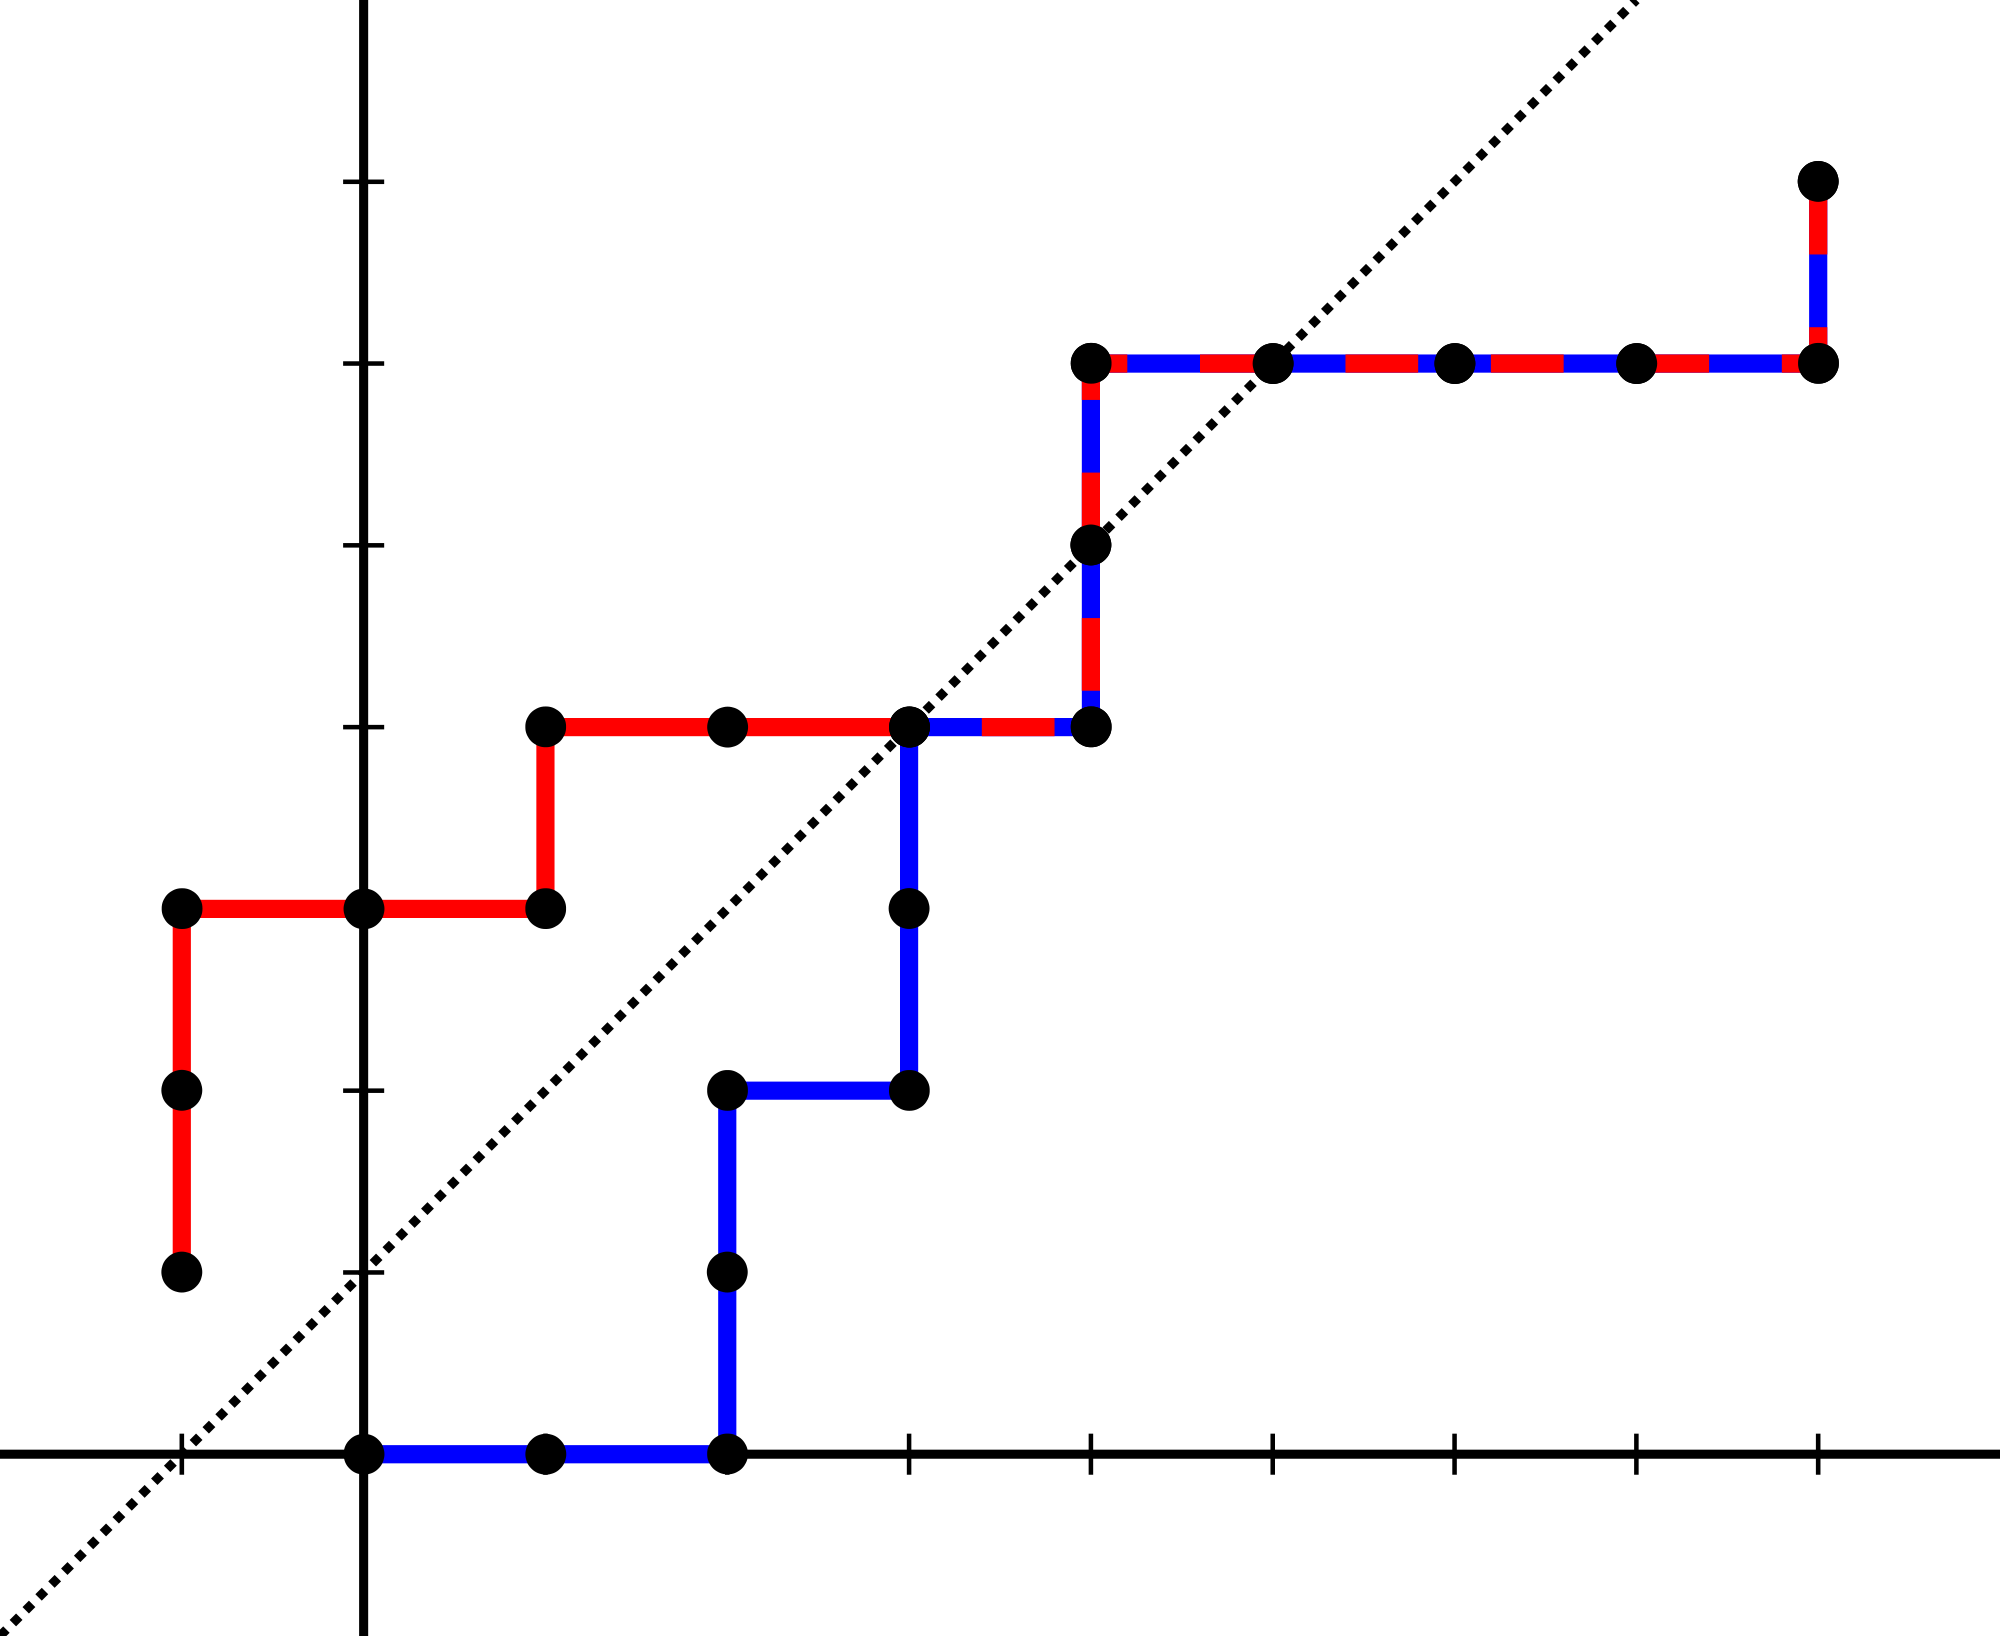
\includegraphics[width=150pt]{2000px-AndreReflection.png}
%	\caption{Bertrand's Ballot prob allowing Ties}
%	\label{fig:Bertrand's_Ballot_prob}
%\end{figure}

An interesting application of this is the famous Catalan number formula, which can be introduced under the random walk story. A random walk on the integers is to take $n$ steps of unit length, beginning at the origin and ending at the point $m$, that never become negative. Assuming $n$ and $m$ have the same parity and $n \ge m \ge 0$, this number is, according to the Bertrand's Ballot prob allowing ties,
\begin{equation*}
	{n \choose \frac{n+m}{2}} - {n \choose \frac{n+m}{2}+1} = \frac{m+1}{\frac{n+m}{2}+1} {n \choose \frac{n+m}{2}}
\end{equation*}
Here, $p+q=n$ and $p-q=m$, compared to our used settings. When $m=0$ and $n$ is even, this gives the Catalan number $\frac{1}{\frac{n}{2}+1} {n \choose \frac{n}{2}}$.

Let's tweak this prob a little bit more. Let's say candidate A starts at $a$ ``bonus'' votes, not 0. That is to say, the system goes from $(0,a)$ to $(p+q,p+a-q)$. If we do not allow ties, all paths hit the x-axis will be unfavorable, and the number of these paths equals the number of paths from $(0,a)$ to its ``mirror'' point $(p+q,-p-a+q)$. So, there are in total ${p+q \choose p+a}$ unfavorable paths, and the probability is $1 - \frac{{p+q \choose p+a}}{{p+q \choose p}}$. Note when $a=0$, there is already a tie, and the question really should be asked as: ``What if the first count is A, and then the process never has a tie''. So the probability should compute as:
\begin{equation*}
	1 - \frac{p}{p+q} \frac{{p-1+q \choose p-1}}{{p-1+q \choose p-1}} = \frac{p-q}{p+q}
\end{equation*}
It should have no prob with $a>0$.

If we allow ties, the ``mirror'' point should be reflected against $y=-1$, so it becomes $(p+q,-2-p-a+q)$. Now, suppose we go up $u$ steps and go down $d$ steps. Solving the following equations:
\begin{eqnarray*}
	u+d & = & p+q\\
	u+a-d & = & -2-p-a+q
\end{eqnarray*}
gives us $u=q-a-1$ and $d=p+a+1$. So there are ${p+q \choose p+a+1}$ paths unfavorable, and the probability is then $1-\frac{{p+q \choose p+a+1}}{{p+q \choose p}}$. When $a=0$, this becomes $\frac{p+1-q}{p+1}$, which agrees with what we obtained earlier.

In summary, if one starts at $(0,a)$ and ends at $(p+q,p+a-q)$, the number of unfavorable paths is $p+q \choose p+a$ if not allowing ties, $p+q \choose p+a+1$ if allowing ties.


\section{Catalan Number}
In chapter \ref{chapter: Bertrand_Ballot_prob}, we first met Catalan number from the generalized Bertrand's Ballot prob. We write here again the definition of Catalan number, with an intuitive interpretation.

The Catalan number is defined as,
\begin{equation}
	C_n = \frac{1}{n+1} {2n \choose n}
\end{equation}
The underlying story reads: Given two urns, one with $n$ red balls and the other with $n$ black balls, we want to draw one ball at a time (either red or black), such that at no time the number of pre-specified color is less than its alternative.

Since the Catalan number is associated with two equal-sized sets, it is oftentimes co-occurrent  with the words "pair", "full binary", and etc. 
\section{Conditional Probability}
\begin{deff}
	If $P(F) > 0$, then
	\begin{equation}
		P(E|F) = \frac{P(E,F)}{P(F)}
	\end{equation}
	$P(E|F)$ is called the conditional probability of $E$ given $F$. Conditional probability agrees with Definition \ref{def:probability}, and should be treated in the same way.
\end{deff}

\begin{deff}
	The multiplication rule
	\begin{equation}
		P(E_1, E_2, \ldots, E_n) = P(E_1) P(E_2|E_1) \ldots P(E_n|E_1, \ldots, E_{n-1})
	\end{equation}
\end{deff}

\begin{deff}
	Bayes' Formula
	\begin{equation}
		P(A_i|B) = \frac{P(B|A_i)P(A_i)}{P(B)}
	\end{equation}
	where $P(A_i)$ is sometimes called the prior distribution, $P(B|A_i)$ the likelihood function, and $P(A_i|B)$ the posterior distribution. The partition function $P(B)$ can be computed using the law of total probability
	\begin{equation}
		P(B) = \sum^n_{j=1}P(B|A_j)P(A_j)
	\end{equation}
\end{deff}

\begin{deff}
	Two events $E$ and $F$ are said to be {\em{independent}} if	
	\begin{equation}
		P(E,F) = P(E)P(F)
	\end{equation}
	A set of events are independent if every finite subset of these events is independent.
\end{deff}

\section{Conditional Probability}
\section{Conditional Expectation}
\section{Conditional Independence} 
\section{Probaility Space}
\section{Sample Space, Events, and Probability}
\begin{deff}
	A sample space $S$ is a set of all possible outcomes of an experiment. An outcome is also called a sample point.
\end{deff}
Note, when an experiment consists of several repetitions, each one of them is called a {\em{trial}}. As an example, if one decides to toss a coin 42 times, we can call each toss a trial of the experiment composed of 42 ones.

\begin{deff}
	An event $E$ is a subset of the sample space $S$. If the outcome of the experiment is contained in $E$, then we say that $E$ occurred.
\end{deff}

\begin{deff}\label{def:probability}
In short, a probability space is a measure space such that the measure of the whole space is equal to one. The expanded definition is following: a probability space is a triple $(\Omega,\; \mathcal{F},\; P)$ consisting of:
\begin{itemize}
\item the sample space $\Omega$ --- an arbitrary non-empty set,
\item the $\sigma-algebra$ $\FF \in 2^\Omega$ (also called $\sigma-filed$) --- a set of subsets of $\Omega$, called events, such that:
	\begin{itemize}
	\item $\FF$ contains the empty set: $\emptyset \in \FF$,
	\item $\FF$ is closed under complements: if $A \in \FF$, then also $(\Omega \setminus A) \in \FF$,
	\item $\FF$ is closed under countable unions: if $A_i \in \FF$ for $i=1,2,\ldots$, then also ($\bigcup A_i) \in \FF$,
	\end{itemize}
\item the probability measure $P: \FF \rightarrow [0,1]$ --- a function on $\FF$ such that:
\item $P$ is countably additive: if $\{A_i\} \in \FF$ is a countable collection of pairwise disjoint sets, then $P(\bigcup A_i) = \sum P(A_i)$, where $\bigcup$ denotes the disjoint union,
\item the measure of entire sample space is equal to one: $P(\Omega)=1$.
\end{itemize}
\end{deff}

\section{Probability Axioms}
\subsection{Law of Total Probability}
Suppose $B_n (n=1,2,3,\cdots$ is a finite or countably infinity partition of the sample space, then for an event $A$
\begin{align}
	Pr(A) = \sum_n Pr(A,B_n)
\end{align}
or,
\begin{align}\label{eq:Law of Total Probability}
	Pr(A) = \sum_n Pr(A|B_n) Pr(B_n)
\end{align}
It can also be stated for conditional probabilities. Suppose $X$ is an event in the same sample space, we have
\begin{align}
	Pr(A|X) = \sum_n Pr(A|B_n,X)Pr(B_n|X)
\end{align}
One application of Eq~\ref{eq:Law of Total Probability} is when calculating $Pr(A)$ is difficult, we can introduce an ``auxiliary variable'' $B$, in the hope that the conditional probability $Pr(A|B_n)$ is easier to compute.
\subsection{Law of Total Variance}
\subsection{Law of Total Covariance}
\subsection{Law of Total Expectation}
\subsection{Law of Total Cumulance}
\subsection{Probability Inequalities}

\section{Types of Probabilities: Frequentism and Bayesian} 
\section{Random Variables}
The Laplace distribution can be written as an infinite mixture of Gaussians with variance $w$ distribution according to an exponential distribution. An exponential distribution can be written as a $\chi^2$ distribution with two degrees of freedom.
\section{Continuous Random Variables}
\section{Discrete Random Variables}
\section{Joint Distributed Random Variables}
\section{Random Vectors/Matrices}
\section{Function of Random Variables}
\subsection{Transformation}
\subsection{Convolutions: Sum of Normally Distributed Random Variables}
\subsection{Product Distribution}
\subsection{Ratio Distribution} 
\chapter{Useful Distributions}
\section{Discrete Distributions}
\subsection{Poisson Distribution}
\subsection{Bernoulli Distribution}
\subsection{Binomial Distribution}
\subsection{Negative Binomial Distribution}
\subsection{Categorical Distribution}
\subsection{Multinomial Distribution}
\subsection{Geometric Distribution}
\subsection{Hyper-Geometric Distribution}
\subsection{Poisson Distribution}
\section{Continuous Distributions}
\subsection{Uniform Distribution}
\subsection{Exponential Distribution}
\subsection{$\chi^2$ Distribution}

\subsection{Gaussian Distribution}
\subsubsection{Univariate Gaussian}
\subsubsection{Multivariate Gaussian}
\begin{align}
	f(\x|\bmu,\bSigma) = \frac{1}{\sqrt{2\pi|\bSigma|}} \exp\left\{-\frac{1}{2}(\x-\bmu)^T\bSigma^{-1}(\x-\bmu)\right\}
\end{align}
Using the technique of `completing the square', we have
\begin{align}
	f(\x_1|\x_2) &= \frac{f(\x_1,\x_2)}{f(\x_2)}\\
	&= \frac{1/\sqrt{2\pi|\bSigma|}\exp\left\{-\frac{1}{2}(\x-\bmu)^T\bSigma^{-1}(\x-\bmu)\right\}}{1/\sqrt{2\pi|\bSigma_{22}|}\exp\left\{-\frac{1}{2}(\x_2-\bmu)^T\bSigma_{22}^{-1}(\x_2-\bmu)\right\}}\\
	&= C \cdot \exp\left\{-\frac{1}{2}(\x-\bmu)^T\bSigma^{-1}(\x-\bmu)\right\}\\
	&= C \cdot \exp\left\{-\frac{1}{2}[(\x_1-\bmu_1)^T\bLambda_{11}(\x_1-\bmu_1)+(\x_1-\bmu_1)^T\bLambda_{12}(\x_2-\bmu_2)+(\x_2-\bmu_2)^T\bLambda_{21}(\x_1-\bmu_1)]\right\}\\
	&= C \cdot \exp\left\{-\frac{1}{2}\x_1^T\bLambda_{11}\x_1 + \x_1^T[\bLambda_{11}\bmu_1 - \bLambda_{12}(\x_2-\bmu_2)]\right\}	
\end{align}
Hence
\begin{align}
	\bSigma_{1|2} &= \bLambda_{11}^{-1}\\
	\bmu_{1|2} &= \bmu_1 - \bLambda_{11}^{-1}\bLambda_{12}(\x_2-\bmu_2)
\end{align}
or
\begin{align}
	\bSigma_{1|2} &= \bSigma_{11} - \bSigma_{12}\bSigma_{22}^{-1}\bSigma_{21}\\
	\bmu_{1|2} &= \bmu_1 + \bSigma_{12}\bSigma_{22}^{-1}(\x_2-\bmu_2)
\end{align}

\subsection{Dirichlet Distribution}
\subsubsection{Gamma Function and Beta Function}
The {\em{gamma function}} is defined for all complex numbers except the non-positive integers. For complex numbers with a positive real part, it is defined via an improper integral that converges:
\begin{equation}
	\Gamma(z) = \int_0^\infty e^{-t} t^{z-1} dt
\end{equation}
For all positive numbers $z$,
\begin{equation}
	\Gamma(z) = (z-1)\Gamma(z-1)
\end{equation}
and in particular, if $n$ is a positive integer:
\begin{equation}
	\Gamma(n) = (n-1)!
\end{equation}
Note, the gamma function shifts the normal definition of factorial by 1.

The {\em{beta function}} is defined by
\begin{equation}
	B(x,y) = \int_0^1 t^{x-1} (1-t)^{y-1} dt
\end{equation}
for $Re(x), Re(y) > 0$.

It can also be written as
\begin{equation}
	B(x,y) = \frac{\Gamma(x) \Gamma(y)}{\Gamma(x+y)}
\end{equation}

\subsubsection{Introduction}
The Dirichlet distribution of order $K \ge 2$ with parameters $\alpha_1, \dots, \alpha_K > 0$ has a probability density function with respect to Lebesgue measure on the Euclidean space $\RR^{K-1}$ given by
\begin{equation}
	f(x_1, \dots, x_{K-1}; \alpha_1, \dots, \alpha_K) = \frac{1}{B(\balpha)} \prod^K_{i=1} x_i^{\alpha_i-1}
\end{equation}
for all $x_1, \dots, x_K > 0$ and $x_1 + \dots + x_K = 1$. The density is zero outside this open\footnote{``Open'' here means none of the $x_i$'s can be 1, actually $x_i \in (0,1)$.} $(K-1)$-dimensional simplex.

The normalizing constant is the multinomial beta function, which can be expressed in terms of the gamma function:
\begin{equation}
	B(\balpha) = \frac{\prod_{i=1}^K \Gamma(\alpha_i)}{\Gamma(\sum_{i=1}^K \alpha_i)}, \mbox{ where } \balpha=(\alpha_1, \dots, \alpha_K)
\end{equation}


\subsection{$t$ Distribution}
\subsection{Inverse Gaussian Distribution}
\subsection{log-normal Distribution}
\subsection{Laplace Distribution}
\subsection{Beta Distribution}
\subsection{Gamma Distribution}
\subsection{Wishart Distribution}
\section{Quantitative Measure and Characteristic Functions}
\section{Describing Shape of a Distribution: Skewness, Kurtosis}
\section{Describing a Sample: Mean, Variance}
\section{Degrees of Freedom, Mean, Variance, and Moment, Central Moment, Cumulant, Law of the unconscious statistician}
\section{Percentile and Median}
\section{Coefficient of Variation}
\section{Covariance and Correlation}
\section{Moment Generating Function}
\section{Characteristic Function}

\section{Limit Theorems}
\section{Markov and Chebyshev Inequalities}
\begin{thm}
	{\underline{Markov's Inequality}}. If $X$ is a random variable that takes only nonnegative values, then for any value $a > 0$, $$P\{X \ge a\} \le \frac{E[X]}{a}$$
\end{thm}

\begin{thm}
	{\underline{Chebyshev's Inequality}}. If $X$ is a random variable with finite mean $\mu$ and variance $\sigma^2$, then, for any value $k > 0$, $$P\{|X-\mu| \ge k\} \le \frac{\sigma^2}{k^2}$$
\end{thm}

\section{Weak Law of Large Numbers}
\begin{thm}
	{\underline{The Weak Law of Large Numbers}}. Let $X_1, X_2, \cdots$ be a sequence of i.i.d. random variables, each having finite mean $E[X_i] = \mu$. Then, for any $\epsilon > 0$, $$P\left\{\left|\frac{X_1+\cdots+X_n}{n} - \mu\right| \ge \epsilon \right\} \to 0 \mbox{ as } n \to \infty$$
\end{thm}

\section{Central Limit theorem}
\begin{thm}
	{\underline{Central Limit theorem}}. Let $X_1, X_2, \cdots$ be a sequence of independent and identically distributed random variables, each having mean $\mu$ and variance $\sigma^2$. Then the distribution of $$\frac{\frac{X_1+\cdots+X_n}{n}-\mu}{\sqrt{\sigma^2/n}} = \frac{X_1+\cdots+X_n - n\mu}{\sigma \sqrt{n}}$$ tends to the standard normal as $n \to \infty$.
\end{thm} 
\section{Selected Topics of Probability}
\section{Indicator Variables}
\section{Ordered Statistics}
\section{Copula}
\section{coupling}
\section{The Reflection Principle}



\newpage
\part{Elementary Theory of Stochastic Processes}
%!TEX root = ../Probability.tex

\chapter{Introduction}
\deff{
	A \emph{stochastic process} is a collection of random variables $X(t)$ for $t \in T$, where the \emph{time} parameter $T$ is usually\footnote{It can be defined in a general space.} a subset of $\RR$. The set $\mathscr{S}$ containing all possible values of $X(t)$ is called the \emph{state space} of the process.
}

There are four common types of stochastic processes (with corresponding examples):
\begin{table}[h]
\centering
  \begin{tabular}{ | c | c | c | }
    \hline
     & \textbf{Finite or Countable State Space} & \textbf{Continuous State Space} \\ \hline
    \textbf{Discrete Time} & Markov Chains & Harris Chains \\ \hline
    \textbf{Continuous Time} & Poisson Processes and Hawkes Processes & Gaussian Processes and Wiener Processes \\ \hline    
  \end{tabular}
  \small{\caption{Four Common Types of Stochastic Processes.}}
\end{table}

\deff{
	A {\em{renewal process}} is an idealized stochastic model for events that occur randomly in time (generically called renewals or arrivals). The basic mathematical assumption is that the times between the successive arrivals are independent and identically distributed (i.i.d.). 
}

\deff{
	A {\em{delayed renewal process}} is just like an ordinary renewal process, except that the first arrival time is allowed to have a different distribution than the other inter-arrival times.
}


\deff{
	A {\em{counting process}} is a stochastic process $\{N(t), t \ge 0\}$ with values that are non-negative, integer, and increasing:
}

\deff{
	A {\em{point process}} is a collection of mathematical points randomly located on some underlying mathematical space such as the real line, the Cartesian plane, or more abstract spaces.
}

\deff{
	A {\em{diffusion process}} is a solution to a stochastic differential equation. For example, Brownian motion.
}

\deff{
	A {\em{jump process}} is a type of stochastic process that has discrete movements, called jumps, with random arrival times, rather than continuous movement, typically modeled as a simple or compound Poisson process.
}
\chapter{Markov Chains}
\section{Introduction}
\deff{
The \emph{Markov property} is defined by the requirement that
\begin{align}
	P(X_{n+1}=x_{n+1} \vert X_0=x_0,\cdots,X_n=x_n) = P(X_{n+1}=x_{n+1} \vert X_n=x_n)
\end{align}
}
\deff{
	The conditional probabilities $P(X_{n+1}=y \vert X_n=x)$ are called the \emph{transition probabilities} of the chain.
}

\deff{
	We say a Markov chain has \emph{stationary transition probabilities} if the transition probabilities $P(X_{n+1}=y \vert X_n=x)$ is independent of the time $n$.
}

From now on, when we say that $X_n, n \ge 0$ forms a Markov chain, we mean that these random variables satisfy the Markov property and have stationary transition probabilities.

\deff{
	A state $a$ of a Markov chain is called an \emph{absorbing state} if $P(a,a) = 1$ or, equivalently, if $P(a,y) = 0$ for all $y \ne a$.
}

\section{Discrete Time Markov Chains}
\subsection{Gambler's Ruin}
\subsection{Discrete Time Branching Processes}

\section{Continuous Time Markov Chains}

\section{Poisson Processes}
\section{Poisson Processes on the Line}
\section{Variable Rate Poisson Processes}
\section{Poisson Processes in Higher Dimensions} 
\chapter{Renewal Theory}   
\section{Renewal theory for positive lattice valued random variables as connected with Markov chains: Blackwell's renewal theorem for positive lattice valued random variables}   
\section{Selected Topics of Stochastic Processes}
\section{Martingales which are functions of discrete time Markov chains}
\section{Brownian motion: Path properties, reflection principle, random walk approximation.}
\section{Random Fields}
\section{Discrete and Continuous Time Birth and Death processes}
\section{Discrete and Continuous Time Queuing processes}
\section{Finite State Space Pure Jump Processes}
\section{Infinite Server Queue}


\newpage
\part{Measure-theoretical Probability}
\chapter{Introduction}
\section{Why Do We Need Rigorous Probability Theory?}
Let's recall the axioms from non-measure probability courses. We have a \emph{sample space} $\Omega$, the elements of which $w \in \Omega$ called \emph{outcomes}, and the subsets $E \subset \Omega$ called \emph{events}. \emph{Probability measure} is nothing but assigning probability $P(E)$ to each event $E \subset \Omega$, under the following constraints:
\begin{enumerate}
	\item $P(E) \in [0,1]$
	\item $P(\Omega) = 1$
	\item $P(\uplus_{i=1}^\infty E_i) = \sum_{i=1}^n P(E_i)$
\end{enumerate}
where in the last constraint, `$\uplus$' means the union of \emph{disjoint} sets.

One of the motivations\footnote{Add unification of discrete and continuous r.v's.} of developing measure-theoretical probability theory is triggered by the following question:

\vspace{2 mm}
\textbf{Q: \emph{How do we know the three listed axioms are consistent, in particular, the last constraint?}}
\vspace{0.5 mm}

Actually, the \emph{Banach-Tarski paradox} and the \emph{Vitali paradox} are such counter examples (TBA). We have two choices: either we could reject the \emph{axiom of choice}, which is one of the basic assumptions made in the two paradoxes; or we could claim there are some subsets $E \subset \Omega$ that is `non-measurable'. In this course, we take the second solution.

\section{Normal Numbers}
\deff{
	Every $X \in [0,1]$ has a binary decimal expansion $X = 0.d_1d_2d_3\cdots$ or $X = \sum_{k=1}^\infty d_k 2^{-k}$, $d_k \in \{0,1\}$. However, it is possible that $X$ may have two expansions, for example, $X=0.111\cdots = 0.1000\cdots$. We choose the expansion ending in all 1's to make it well-defined.
}

\deff{
	$X \in (0,1)$ is normal if $\lim\limits_{n \to \infty} \frac{1}{n} \sum_{k=1}^n d_k = \frac{1}{2}$.
}

\prop{
	If $X \sim U(0,1)$, then $P(X\mbox{ is normal}) = 1$.
}

\lem{
	Suppose that $X_1, X_2, \cdots$ are i.i.d $Ber(1/2)$. Then $X = \sum_{n=1}^\infty X_n 2^{-n}$ is uniform on $(0,1)$.
}
\prof{	
	We (only) need to show $P(X \in (a,b]) = b - a$.\\
	
	Case 1: $\exists k, s.t. (a,b] = ((k-1)2^{-n}, k2^n]$. Since $(k-1)2^{-n} = 0.d_1d_2 \cdots d_n000\cdots$,
	\begin{align}
		P(X \in ((k-1)2^{-n},k2^{-n}]) &= P(X_1=d_1,X_2=d_2,\cdots,X_n=d_n, X_i=1 for i > n) = 2^{-n} = b-a
	\end{align}

	Case 2: $(a,b] = (l2^{-n},k2^{-n}], l < k$.
	\begin{align}
		P(X \in (l2^{-n},k2^{-n}]) &= (k-l)2^{-n} = b- a
	\end{align}

	In general, if $a < b$, let $a_n, b_n \in 2^{-n}\Z$ be s.t. $a_n \le a < a_n + 2^{-n}, b_n - 2^{-n} \le b < b_n$, then
	\begin{align}
		P(X \in (a,b]) \le P(X \in (a_n,b_n]) = b_n - a_n
	\end{align}
	$b_n - a_n - 2^{-n+1} = P(X \in (a_n+2^{-n},b_n-2^{-n}) \le \epsilon$. Note, $b-a \le b_n - a_n \le b- a + 2^{-n+1}$.

	We need to show that $P(\lim\limits_{n \to \infty} \frac{1}{n} \sum_{k=1}^\infty = \frac{1}{2}) = 1$. This is the SLLN.
}

We know that $\{X \in (a,b]\}$ are events. Why is $\{X\mbox{ is normal}\}$ an event?
\begin{align}
	\{X\mbox{ is normal}\} = \left\{\lim\limits_{n \to \infty} \frac{1}{n} \sum_{k=1}^\infty = \frac{1}{2}\right\} = \bigcap_{l=1}^\infty \bigcup_{m=l}^\infty \bigcap_{n=m}^\infty \left\{\left\vert \frac{1}{n} \sum_{k=1}^\infty - \frac{1}{2} \right\vert < \frac{1}{l} \right\}
\end{align}
This is equivalent to $\forall \epsilon = \frac{1}{l} > 0, \exists m < \infty, s.t., |\frac{1}{n} \sum_{k=1}^\infty - \frac{1}{2}| < \epsilon, \forall n \ge m$.

\section{Formal Definition of Probability Space}
\deff{
	A collection $\FF$ of subsets of $\Omega$ is a $\sigma$-field (or algebra) if
	\begin{enumerate}
		\item $\FF$ is non-empty;
		\item If $A \subset \FF$, then $A^c \in \FF$ (closed under complement);
		\item If $\{A_i\}$ is a countable sequence of elements of $\FF$, then $\cup_i A_i \in \FF$ (closed under countable unions).
	\end{enumerate}	
}
Note, 1) $\Omega \in \FF, \emptyset \in \FF$ since $\Omega = A \cup A^c if A \in \FF$. $\emptyset = \Omega^c$. 2) $\FF$ is closed under countable intersections.

\deff{
	A \emph{measure space} is a pair $(\Omega, \FF)$ where $\FF$ is a $\sigma$-field of subsets of $\Omega$.
}

\deff{
	A non-negative measure $\mu$ on $(\Omega, \FF)$ is a function $\mu: \FF \to \bar \RR_+ = [0,\infty]$ s.t.
	\begin{enumerate}
		\item $\mu(\emptyset) = 0$;
		\item If $A_i$ is a sequence of disjoint sets in $\FF$, then $\mu(\uplus_{i=1}^\infty A_i) = \sum_{i=1}^\infty \mu(A_i)$.
	\end{enumerate}
}

\deff{
	A \emph{probability space} is a triple $(\Omega, \FF, P)$ where $(\Omega, \FF)$ is a measure space, and $P$ is a measure on $(\Omega, \FF)$ with $P(\Omega) = 1$.
}

\ex{
	$\FF = 2^{\Omega}$ (all subsets of $\Omega$). If $\Omega = \Z$, then usually, $\FF = 2^\Omega$ is the $\sigma$-field we use. If $\Omega=(0,1]$ or $\R$, then $\FF$ is usually too big.
}

\ex{
	Let $\AA \subset 2^\Omega$, then $\sigma(\AA)$ is the smallest $\sigma$-field containing $\AA$. If $\OO \subset \R$ is the collection of all open subsets of $\R$, then $\sigma(\OO) = \BB$ is called the \emph{Borel $\sigma$-field}.
}

\chapter{Lecture 5 (1/21/2015 Wednesday): }
(Today and Friday) in Appendix A.
\deff{
	A non-empty collection of subsets $\AA \subset 2^\Omega$ is called an algebra if
	\begin{enumerate}
		\item $A \in \AA$ then $A^c \in \AA$
		\item $A, B \in \AA$ then $A \cup B \in \AA$
		\item $A, B \in \AA$ then $A \cap B \in \AA$
	\end{enumerate}
}

\deff{
	$\mu: \AA \rightarrow [0,\infty]$ is a measure on the algebra $\AA$ if
	\begin{enumerate}
		\item $\mu(\emptyset) = 0$
		\item If $\uplus_{i=1}^\infty A_i \in \AA$ then $\mu(\uplus_{i=1}^\infty A_i) = \sum_{i=1}^\infty \mu(A_i)$
	\end{enumerate}
}

\deff{
	A measure $\mu$ is $\sigma$-finite (on an algebra or a $\sigma$-field) if $\exists$ a sequence $A_n \nearrow \Omega$ with $\mu(A_n) < \infty$ ($A_n \subset A_{n+1}$ and $\Omega = \cup_{i=1}^\infty A_n$)
}

\begin{thm}
	(Caratheodory Extension) Let $\mu$ be a $\sigma$-finite measure on an algebra $\AA$. Then $\mu$ has a unique extension to a measure on $(\Omega, \sigma(\AA))$.
\end{thm}

Note: Meausre on algebras also satisfy Themorem 1.1.1
\begin{enumerate}
	\item $A \subset B$ then $\mu(A) \le \mu(B)$
	\item $\mu(\cup_{i=1}^\infty A_i \le \sum_i \mu(A_i)$ if $\cup A_i \in \AA$
\end{enumerate}


\chapter{Probability Space and Measure}

\section{Algebra of Sets}

\subsubsection{Set Operations}
Given two sets $A, B \in \Omega$, there are four basic binary operations on sets:
\begin{enumerate}
	\item {\em{Union}}: $A \cup B = \{x: x \in A \mbox{ or } x \in B\}$
	\item {\em{Intersection}}: $A \cap B = \{x: x \in A \mbox{ and } x \in B\}$
	\item {\em{Set difference}}: $A \setminus B = \{x: x \in A \mbox{ and } x \notin B\}$
	\item {\em{Set complement}}: $A^c = \Omega \setminus A$
\end{enumerate}

Set complement is the ``strongest'' operation, because if a collection of sets $\AA$ is closed under complement, and if it is also closed under any one of the other three operations, $\AA$ is closed under the rest two. That is seen from,
\begin{align}
	\mbox{If closed under } union &
	\begin{cases}
		A \cap B = (A^c \cup B^c)^c\\
		A \setminus B = A \cap B^c = (A^c \cup B)^c
	\end{cases}	
	\\
	\mbox{If closed under } intersection &
	\begin{cases}
		A \cup B = (A^c \cap B^c)^c\\		
		A \setminus B = A \cap B^c
	\end{cases}
	\\
	\mbox{If closed under } difference &
	\begin{cases}
		A \cap B = A \setminus (A \setminus B)\\
		A \cup B = (A^c \cap B^c)^c = (A^c \setminus (A^c \setminus B^c))^c\\
	\end{cases}		
\end{align}

The difference operation is the second ``strongest'' operation, in that if a collection of sets $\AA$ is closed under difference, it is closed under intersection, that is seen from,
\begin{align}
	A \cap B = A \setminus (A \setminus B)
\end{align}

The third ``strongest'' operation is the union, which can not be implied from difference or intersection, or their combination.

The ``weakest'' operation is the intersection, which can be implied from the difference.

To summarize, the ``strongest'' pair would be the complement plus any one more, which implies everything else; the second ``strongest'' would be the difference plus the union, which implies the intersection but not the complement ($\Omega$ may not be in the collection). \smallmarginpar{\textdbend}

\subsubsection{Class of Set Collection}
\begin{deff}
	Given a set $\Omega$, a non-empty collection $\PP \subset 2^\Omega$ is called a {\em{$\pi$-system}} iff:
	
	\center{$\forall A, B \in \PP$, $A \cap B \in \PP$}
\end{deff}
Notice, this has the weakest requirement.

\begin{deff}
	Given a set $\Omega$, a non-empty collection $\QQ \subset 2^\Omega$ is called a {\em{semiring}} iff:
	
	\center{$\forall A, B \in \QQ \mbox{ and } A \supset B$}
	\center{$\exists C_k \subset \QQ, s.t., A \setminus B = \bigcup_{k=1}^n C_k$}
\end{deff}

\begin{deff}
	Given a set $\Omega$, a non-empty collection $\RR \subset 2^\Omega$ is called a {\em{ring}} iff:
	
	\center{$\forall A, B \in \RR$, $A \cup B \in \RR$ and $B \setminus A \in \RR$}
\end{deff}

There are two points need to mention: the empty set is in a ring, since $A \setminus A = \emptyset$; $\AA$ is also closed under intersection (the reverse need not be true).

\begin{deff}
	A {\em{ring}} $\AA$ is called an {\em{field}} iff $\Omega \in \AA$.
\end{deff}
So a field is closed under all {\em{finite}} combination of set operations.


\begin{deff}
	An {\em{field}} is called a {\em{$\sigma$-field}} if for any sequence ${A_n}$ of sets in $\AA$, $\cup_{n \ge 1} A_n \in \AA$.
\end{deff}

$\not \exists$

\chapter{Integration Theory}
\chapter{Random Variables}
\chapter{Law of Large Numbers}
\section{Types of Convergence}
\subsubsection{Convergence in Distribution}
\subsubsection{Convergence in Probability}
\subsubsection{Almost Surely Convergence}
\subsubsection{$L^p$ Convergence}

\section{Weak Law of Large Numbers (WLLN)}
\section{Strong Law of Large Numbers (SLLN)}

\chapter{Central Limit theorem}

\chapter{Some Tricks}
\section{Prove by Contraposition}

\section{Construct Finer Partition}
Given twofinite partitions $\{A_n\}$ and $\{B_m\}$, a finer partition can be constructed as
\begin{align*}
	(\cup_{i=1}^n A_i) \bigcap (\cup_{j=1}^m B_j) = \bigcup (\cap_{i=1}^n \cap_{j=1}^m A_i B_j)
\end{align*}

\section{Prove Equality}
To prove two numerical quantities are equal $X=Y$, often times we can do this by showing $X \le Y$ and $X \ge Y$. Similarly, to prove two sets are equal $E = F$, we can show $E \subset F$ and $E \subset F$.

\section{An Epsilon of Room}
If one has to show that $X \le Y$, try proving that $X \le Y + \epsilon, \forall \epsilon > 0$. This trick combines well with the ``Prove Equality'' trick.

In a similar spirit, if one needs to show that a quantity $X$ vanishes, try showing that $|X| \le \epsilon, \forall \epsilon > 0$.

If one wants to show that a sequence $x_n$ of real numbers converges to zero, try showing that $\limsup_{n \to \infty} |x_n| \le \epsilon, \forall \epsilon > 0$

{\textbf{One caveat:}} for finite $x$, and any $\epsilon > 0$, it is true that $x + \epsilon > x$ and $x - \epsilon < x$, but it is not true when $x$ is equal to $+\infty$ or $-\infty$. \smallmarginpar{\textdbend}


\section{Interpretations of Probability}
\subsection{Cox's theorem}
\subsection{Principle of Maximum Entropy}

\part{Measure-theoretical Stochastic Processes}

\part{Appendix}

\end{document} 






